\documentclass[letterpaper,11pt]{article}

\usepackage{latexsym}
\usepackage[empty]{fullpage}
\usepackage{titlesec}
\usepackage{marvosym}
\usepackage[usenames,dvipsnames]{color}
\usepackage{verbatim}
\usepackage{enumitem}
\usepackage[hidelinks]{hyperref}
\usepackage{fancyhdr}
\usepackage[english]{babel}
\usepackage{tabularx}
\usepackage{fontawesome5}
\usepackage{multicol}
\setlength{\multicolsep}{-3.0pt}
\setlength{\columnsep}{-1pt}
\input{glyphtounicode}

%new packages

\usepackage{fontenc}
\usepackage{amsmath}
\usepackage{amssymb}
\usepackage{graphicx}



%----------FONT OPTIONS----------

\pagestyle{fancy}
\fancyhf{} % clear all header and footer fields
\fancyfoot{}
\renewcommand{\headrulewidth}{0pt}
\renewcommand{\footrulewidth}{0pt}

% Adjust margins
\addtolength{\oddsidemargin}{-0.6in}
\addtolength{\evensidemargin}{-0.5in}
\addtolength{\textwidth}{1.19in}
\addtolength{\topmargin}{-.7in}
\addtolength{\textheight}{1.4in}

\urlstyle{same}

\raggedbottom
\raggedright
\setlength{\tabcolsep}{0in}

% Sections formatting
\titleformat{\section}{
  \vspace{-4pt}\scshape\raggedright\large\bfseries
}{}{0em}{}[\color{black}\titlerule \vspace{-5pt}]



% Ensure that generate pdf is machine readable/ATS parsable
\pdfgentounicode=1

%-------------------------
% Custom commands
\newcommand{\resumeItem}[1]{
  \item\small{
    {#1 \vspace{-2pt}}
  }
}

\newcommand{\classesList}[4]{
    \item\small{
        {#1 #2 #3 #4 \vspace{-2pt}}
  }
}

\newcommand{\resumeSubheading}[4]{
  \vspace{-2pt}\item
    \begin{tabular*}{1.0\textwidth}[t]{l@{\extracolsep{\fill}}r}
      \textbf{#1} & \textbf{\small #2} \\
      \textit{\small#3} & \textit{\small #4} \\
    \end{tabular*}\vspace{-7pt}
}

\newcommand{\resumeSubSubheading}[2]{
    \item
    \begin{tabular*}{0.97\textwidth}{l@{\extracolsep{\fill}}r}
      \textit{\small#1} & \textit{\small #2} \\
    \end{tabular*}\vspace{-7pt}
}

\newcommand{\resumeProjectHeading}[2]{
    \item
    \begin{tabular*}{1.001\textwidth}{l@{\extracolsep{\fill}}r}
      \small#1 & \textbf{\small #2}\\
    \end{tabular*}\vspace{-7pt}
}


\newcommand{\resumeSubItem}[1]{\resumeItem{#1}\vspace{-4pt}}

\renewcommand\labelitemi{$\vcenter{\hbox{\tiny$\bullet$}}$}
\renewcommand\labelitemii{$\vcenter{\hbox{\tiny$\bullet$}}$}

\newcommand{\resumeSubHeadingListStart}{\begin{itemize}[leftmargin=0.0in, label={}]}
\newcommand{\resumeSubHeadingListEnd}{\end{itemize}}
\newcommand{\resumeItemListStart}{\begin{itemize}}
\newcommand{\resumeItemListEnd}{\end{itemize}\vspace{-5pt}}


\begin{document}
\fontfamily{cmr}\selectfont
\begin{center}
\parbox{3.0cm}{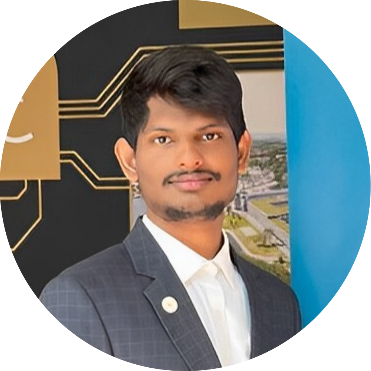
\includegraphics[width=2.7cm,clip]{images/resume_pic_m.png}}
\parbox{\dimexpr\linewidth-3.8cm\relax}{
\vspace{-20pt}
\begin{tabularx}{\linewidth}{L r} \\
    {\Huge \scshape Venkata Sai Yakkshit Reddy Asodi} \\
    Berlin, Germany. \\ \vspace{1pt}
    \small \raisebox{-0.1\height}\faPhone\ +91 8179936156 ~ \href{mailto:saiyakkshit2001@gmail.com}{\raisebox{-0.2\height}\faEnvelope\ {saiyakkshit2001@gmail.com}} ~ 
    \href{https://linkedin.com/in/yakkshit/}{\raisebox{-0.2\height}\faLinkedin\ {yakkshit}} ~
    \href{https://yakkshit.com/}{\raisebox{-0.2\height}\faGlobe\ {yakkshit.com}} ~
    \href{https://github.com/yakkshit}{\raisebox{-0.2\height}\faGithub\ {yakkshit}}
    \vspace{-8pt}
\end{tabularx}}
\end{center}

\vspace{-17pt}
%-----------SUMMARY-----------
\section{Summary}
Full Stack Developer specializing in scalable web applications with React, Node.js, and TypeScript. Experienced in designing secure backend APIs and deploying cloud solutions on Microsoft Azure. Proactive, team-oriented, and solution-driven developer passionate about creating innovative SaaS solutions.

%-----------TECHNICAL SKILLS-----------
\section{Technical Skills}
\begin{itemize}[leftmargin=0.15in, label={}]
\small{
\item{\textbf{Languages:} JavaScript (ES6+), TypeScript, Python, HTML5, CSS3.}
\item{\textbf{Frameworks:} React, Node.js, Express, Next.js, MongoDB.}
\item{\textbf{Cloud & DevOps:} Microsoft Azure, Docker, GitLab CI/CD.}
\item{\textbf{Tools:} Git, Postman, Swagger, REST APIs.}
\item{\textbf{Database:} MongoDB, SQL.}}
\end{itemize}

%-----------EXPERIENCE-----------
\section{Experience}
\resumeSubHeadingListStart
\resumeSubheading
{Circleup AG}{Jan 2024 -- July 2024}
{Lead Full Stack Engineer}{Zurich, Switzerland}
\begin{itemize}
\item Developed and maintained scalable web applications using React, TypeScript, and Node.js.
\item Designed RESTful APIs for backend services using Node.js and MongoDB.
\item Deployed and scaled applications on Microsoft Azure.
\item Collaborated with the product team to develop new features and improve existing solutions.
\item Maintained CI/CD pipelines and version control using GitLab.
\end{itemize}

\resumeSubheading
{Cedzlabs}{Mar 2023 -- Dec 2023}
{Full Stack Developer}{India}
\begin{itemize}
\item Built responsive web applications using React, TypeScript, and MongoDB.
\item Developed REST APIs for managing user data and authentication using Node.js.
\item Worked closely with designers to create intuitive user interfaces.
\item Implemented CI/CD pipelines using GitLab for streamlined deployment.
\end{itemize}

%-----------PROJECTS-----------
\section{Projects}
\resumeProjectHeading
{\textbf{AI Resume Tuner} $|$ \emph{Next.js, Azure Cloud, LLMs}}{Aug 2023 -- Present}
\begin{itemize}
\item Built an AI-powered resume tuning application using Next.js and Azure Cloud for scalability.
\item Integrated backend APIs with LLMs for personalized resume recommendations.
\item Utilized Retrieval Augmented Generation (RAG) to enhance resume content.
\end{itemize}

\resumeProjectHeading
{\textbf{Portfolio Website} $|$ \emph{Next.js, AWS}}{Jan 2023}
\begin{itemize}
\item Developed and deployed a personal portfolio website on AWS using Next.js.
\item Integrated secure file storage and encryption for user uploads.
\item Designed a modern UI/UX using Figma and React.
\end{itemize}

%-----------ACHIEVEMENTS-----------
\section{Achievements}
\begin{itemize}
\item Contributed to open-source projects related to web development and cloud deployments.
\item Spearheaded the development of scalable SaaS solutions in fast-paced startup environments.
\item Active participant in hackathons and tech meetups, winning awards for innovative web applications.
\end{itemize}

\end{document}